\documentclass{beamer}
\usepackage{amsmath}
\usepackage[english]{babel} %set language; note: after changing this, you need to delete all auxiliary files to recompile
\usepackage[utf8]{inputenc} %define file encoding; latin1 is the other often used option
\usepackage{csquotes} % provides context sensitive quotation facilities
\usepackage{graphicx} %allows for inserting figures
\usepackage{booktabs} % for table formatting without vertical lines
\usepackage{textcomp} % allow for example using the Euro sign with \texteuro
\usepackage{stackengine}
\usepackage{wasysym}
\usepackage{tikzsymbols}
\usepackage{textcomp}
\newcommand{\bubblethis}[2]{
        \tikz[remember picture,baseline]{\node[anchor=base,inner sep=0,outer sep=0]%
        (#1) {\underline{#1}};\node[overlay,cloud callout,callout relative pointer={(0.2cm,-0.7cm)},%
        aspect=2.5,fill=yellow!90] at ($(#1.north)+(-0.5cm,1.6cm)$) {#2};}%
    }%
\tikzset{face/.style={shape=circle,minimum size=4ex,shading=radial,outer sep=0pt,
        inner color=white!50!yellow,outer color= yellow!70!orange}}
%% Some commands to make the code easier
\newcommand{\emoticon}[1][]{%
  \node[face,#1] (emoticon) {};
  %% The eyes are fixed.
  \draw[fill=white] (-1ex,0ex) ..controls (-0.5ex,0.2ex)and(0.5ex,0.2ex)..
        (1ex,0.0ex) ..controls ( 1.5ex,1.5ex)and( 0.2ex,1.7ex)..
        (0ex,0.4ex) ..controls (-0.2ex,1.7ex)and(-1.5ex,1.5ex)..
        (-1ex,0ex)--cycle;}
\newcommand{\pupils}{
  %% standard pupils
  \fill[shift={(0.5ex,0.5ex)},rotate=80] 
       (0,0) ellipse (0.3ex and 0.15ex);
  \fill[shift={(-0.5ex,0.5ex)},rotate=100] 
       (0,0) ellipse (0.3ex and 0.15ex);}

\newcommand{\emoticonname}[1]{
  \node[below=1ex of emoticon,font=\footnotesize,
        minimum width=4cm]{#1};}
\usepackage{scalerel}
\usetikzlibrary{positioning}
\usepackage{xcolor,amssymb}
\newcommand\dangersignb[1][2ex]{%
  \scaleto{\stackengine{0.3pt}{\scalebox{1.1}[.9]{%
  \color{red}$\blacktriangle$}}{\tiny\bfseries !}{O}{c}{F}{F}{L}}{#1}%
}
\newcommand\dangersignw[1][2ex]{%
  \scaleto{\stackengine{0.3pt}{\scalebox{1.1}[.9]{%
  \color{red}$\blacktriangle$}}{\color{white}\tiny\bfseries !}{O}{c}{F}{F}{L}}{#1}%
}
\usepackage{fontawesome} % Social Icons
\usepackage{epstopdf} % allow embedding eps-figures
\usepackage{tikz} % allows drawing figures
\usepackage{amsmath,amssymb,amsthm} %advanced math facilities
\usepackage{lmodern} %uses font that support italic and bold at the same time
\usepackage{hyperref}
\usepackage{tikz}
\usepackage{tcolorbox}

\usefonttheme[onlymath]{serif} %set math font to serif ones

\definecolor{beamerblue}{rgb}{0.2,0.2,0.7} %define beamerblue color for later use

%%% defines highlight command to set text blue
\newcommand{\highlight}[1]{{\color{blue}{#1}}}


%%%%%%% commands defining backup slides so that frame numbering is correct

\newcommand{\backupbegin}{
   \newcounter{framenumberappendix}
   \setcounter{framenumberappendix}{\value{framenumber}}
}
\newcommand{\backupend}{
   \addtocounter{framenumberappendix}{-\value{framenumber}}
   \addtocounter{framenumber}{\value{framenumberappendix}}
}

%%%% end of defining backup slides

%Specify figure caption, see also http://tex.stackexchange.com/questions/155738/caption-package-not-working-with-beamer
\setbeamertemplate{caption}{\insertcaption} %redefines caption to remove label "Figure".
%\setbeamerfont{caption}{size=\scriptsize,shape=\itshape,series=\bfseries} %sets figure  caption bold and italic and makes it smaller

\newtcolorbox{boxA}{
    fontupper = \bf,
    boxrule = 1.5pt,
    colframe = black % frame color
}

\usetheme{Boadilla}


% --------------------
% Overall information
% --------------------
\title[Economía I]{Economía I \vspace{4mm}
\\ Magistral 18: Distorsiones de mercado III}
\date{}
\author[Franco Riottini]{Riottini Franco}
\vspace{0.4cm}
\institute[]{Universidad de San Andrés} 


\begin{document}

\begin{frame}
\titlepage
\centering

\includegraphics[scale=0.2]{../Figures/logoUDESA.jpg} 
\end{frame}

\begin{frame}{Distorsiones al equilibrio de mercado}
    \begin{itemize}
        \item Por las características de la realidad \vspace{1mm}
        \begin{itemize}
            \item Monopolios naturales (red eléctrica, agua, gas)   
             \vspace{1mm}
            \item Externalidades
             \vspace{1mm}
            \item Bienes públicos
            \vspace{1mm}
            \item Problemas de información
            \begin{itemize}
                \item Atributos ocultos (selección adversa)
                 \vspace{1mm}
                \item Acciones ocultas (moral hazard)
            \end{itemize}        
        \end{itemize}
    \end{itemize}
\end{frame}

\begin{frame}{Asimetrías de información}
    \begin{boxA}
        \centering
        Hay información asimétrica
        cuando una de las partes tiene información de importancia para una
        transacción que la otra parte desconoce.
    \end{boxA}
    \begin{itemize}
        \item Estos casos se enmarcan en el problema del \textbf{Principal-Agente}, donde el principal \textbf{contrata} a un agente para que realice una tarea.
        \item Pero el agente tiene información que el principal no tiene.
        \item Esto es mucho más comun de lo que parece\dots
    \end{itemize}

    \centering
    
\includegraphics[scale=0.1]{../Figures/Tinder_Info_Asim.png}
\end{frame}

\begin{frame}{Selección Adversa}
    Hay dos tipologías de información asimétrica:
    \begin{itemize}
        \item \textbf{Selección adversa}
        \item \textbf{Riesgo moral}
    \end{itemize}
    \begin{boxA}
        \centering
        La llamada selección adversa sucede cuando no conocemos una característica de la contraparte (atributos ocultos).
    \end{boxA}
    \vspace{-2mm}
    \centering
    % 
\includegraphics[scale=0.05]{../Figures/Swiss_Medical_Logo.jpg}
    \vspace{-10mm}
    \begin{itemize}
        \item ¿Por qué las empresas te hacen examenes antes de entrar?
        \item ¿Por qué los bancos te piden una garantía?
    \end{itemize}
\end{frame}

\begin{frame}{Selección Adversa}
    \begin{itemize}
        \item Cuando hay selección adversa, el riesgo (al igual que vamos a ver en riesgo moral) es que el mercado desaparezca.
        \item Veamos un ejemplo clásico: el mercado de los limones de Akerlof.
        \item Dos tipos de autos: buenos y malos, limones.
        \begin{itemize}
            \item Para el vendedor el auto bueno vale 1000 y el malo 500.
            \item Para el comprador el auto bueno vale 1500 y el malo 750.
            \item ¿A cuanto se venden los autos si sabemos cual es cual?
        \end{itemize}
    \end{itemize}
\end{frame}

\begin{frame}{Selección Adversa: Los limones de Akerlof}
    \begin{itemize}
        \small
        \item ¿Cuanto está dispuesto a pagar un comprador? ¿Qué hace el vendedor?
        \item Si piensa que la probabilidad que un auto sea bueno es $\mu$ y que sea malo  $(1-\mu)$ el \textbf{valor esperado} para un auto típico en el mercado sería  
        
        \[\mu 1500 + (1-\mu) 750= 750 + \mu 750\] 
    \end{itemize}

    \centering
    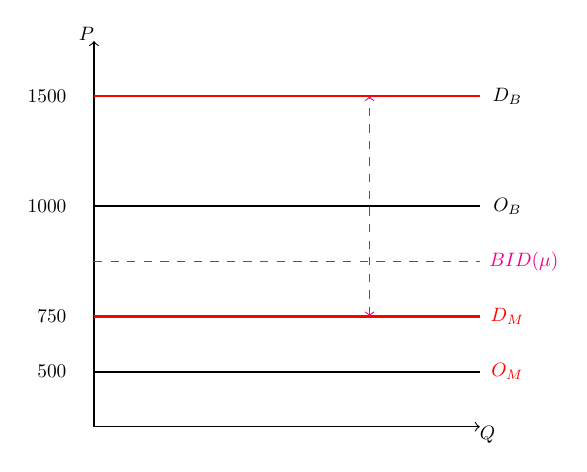
\begin{tikzpicture}[scale=0.7,every node/.style={scale=0.7, inner sep=0, outer sep=0}]

        % Coordenadas de los ejes
        \draw[->, black] (0, 0) -- (7, 0) node[below right] {$Q$}; % Eje x
        \draw[->, black] (0, 0) -- (0, 7) node[above left] {$P$};  % Eje y
        
        % Números de valores en y
        \node[black, anchor=east] at (-0.5, 6) {1500};
        \node[black, anchor=east] at (-0.5, 4) {1000};
        \node[black, anchor=east] at (-0.5, 2) {750};
        \node[black, anchor=east] at (-0.5, 1) {500};
    
        
        % Líneas horizontales
        \draw[thick, black] (0, 1) -- (7, 1);
        \draw[thick, red] (0, 2) -- (7, 2);
        \draw[dashed, magenta] (0, 3) -- (7, 3);
        \draw[thick, black] (0, 4) -- (7, 4);
        \draw[thick, red] (0, 6) -- (7, 6);
        
        % Flecha vertical magenta entre las líneas rosas
        \draw[dashed, magenta, <->] (5, 2) -- (5, 6);
        
        % Textos
        \node[red] at (7.5, 2) {$D_M$};
        \node[red] at (7.5, 1) {$O_M$};
        \node[magenta] at (7.8, 3) {$BID (\mu)$};
        \node[black] at (7.5, 4) {$O_B$};
        \node[black] at (7.5, 6) {$D_B$};
        
    \end{tikzpicture}
\end{frame}

\begin{frame}{Riesgo Moral}
    \begin{boxA}
        \centering
        El riesgo moral sucede cuando no podemos ver el accionar de la contraparte.
    \end{boxA}
    \begin{itemize}
        \item Lo importante acá es que un Agente toma una decisión o realiza una acción que afecta su
        utilidad y la utilidad del Principal.
        \item ¿Contratos laborales atados a objetivos? ¿Pagos en acciones de la empresa?
        \item ¿Garantías? ¿Seguros con deducibles o franquicias?
    \end{itemize}
    \centering
    % 
\includegraphics[scale=0.4]{../Figures/FMI_Riesgo_Moral.jpg}
\end{frame}

\begin{frame}{Riesgo Moral en el Mercado de Seguros}
    \begin{itemize}
        \item En el mercado de seguros, los individuos pueden alterar su nivel de esfuerzo para prevenir riesgos, lo que afecta la prima del seguro. El riesgo moral surge cuando los asegurados reducen su esfuerzo tras obtener cobertura.
        \begin{itemize}
            \item \textbf{Demanda de seguros (D)}: Depende del riesgo de incidente ($p$) y de la cantidad ($Q$).
            \[P = a - \frac{b}{p} Q \]
            \item A medida que aumenta $p$, la demanda se hace más elástica (menos empinada!).
            \item \textbf{Oferta de seguros (O)}: Depende del riesgo de incidente ($p$) y de las cantidades que vendan (aun que esto puede no ser importante).
            \[P = p + c Q \]
            \item A medida que aumenta $p$ cambia la ordenada al origen de la oferta.
            \item Ahora, cuando el esfuerzo baja, el riesgo aumenta...
        \end{itemize}
    \end{itemize}
\end{frame}
    
\begin{frame}
    \frametitle{Riesgo Moral en el Mercado de Seguros}
    \begin{center}
        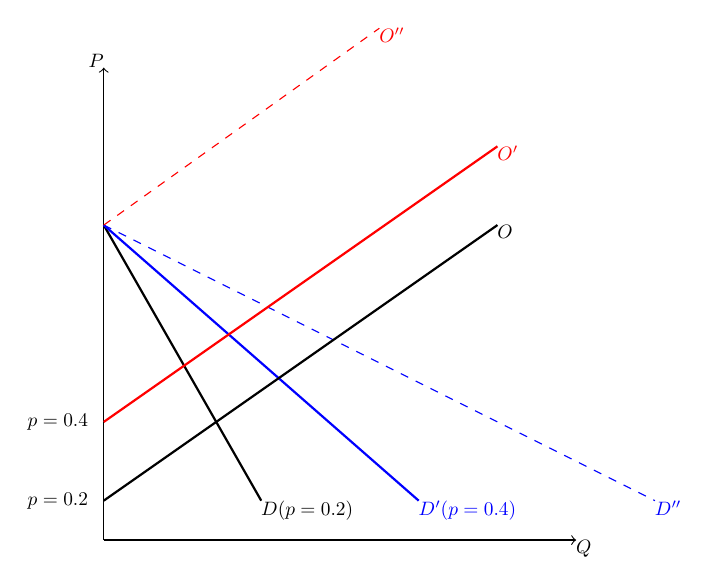
\begin{tikzpicture}[scale=1,every node/.style={scale=0.7, inner sep=0, outer sep=0}]
        % Ejes
        \draw[->] (0,0) -- (6,0) node[below right] {$Q$};
        \draw[->] (0,0) -- (0,6) node[above left] {$P$};
        
        % Curva de Demanda
        \draw[thick, black] (0,4) -- (2,0.5) node[below right] {$D (p = 0.2)$};
        \draw[thick, blue] (0,4) -- (4,0.5) node[below right] {$D' (p = 0.4)$};
        \draw[dashed, blue] (0,4) -- (7,0.5) node[below right] {$D''$};

        % Curva de Oferta
        \draw[thick, black] (0,0.5) -- (5,4) node[below right] {$O$};
        \draw[thick, red] (0,1.5) -- (5,5) node[below right] {$O'$};
        \draw[dashed, red] (0,4) -- (3.5,6.5) node[below right] {$O''$};

        % Números de valores en y
        \node[black, anchor=east] at (-0.2, 0.5) {$p = 0.2$};
        \node[black, anchor=east] at (-0.2, 1.5) {$p = 0.4$};

        % % Etiquetas de puntos
        % \draw[dotted] (3,0) -- (3,3) -- (0,3);
        % \node at (3,-0.3) {C*};
        % \node at (-0.3,3) {P*};
        
        % Punto de equilibrio
        % \node at (3,3) [circle,fill,inner sep=1.5pt]{};
    \end{tikzpicture}
    \end{center}
\end{frame}

\begin{frame}
    \begin{boxA}
        \centering
        Si un individuo que contrata un seguro no hace nada para evitar el
        siniestro, el precio que cobrará la firma aseguradora será tan alto
        que resultará conveniente no contratarlo y el mercado asegurador
        desaparecerá.
    \end{boxA}
\end{frame}

\begin{frame}{Discusiones}
    \begin{itemize}
        \item ¿Por qué pierden valor los autos al salir de la concesionaria?
        \item Políticas de deducibles.
        \item Obama care.
    \end{itemize}
\end{frame}

\begin{frame}{Ejemplos}
    \begin{itemize}
    \item \href{https://www.youtube.com/watch?v=qlg0qakJhKU}{\textbf{Matilda}}
    \item \href{https://www.youtube.com/watch?v=akA8co61He4}{\textbf{Tomates verdes fritos}}
    \item \href{https://www.youtube.com/watch?v=X8BPfLhH6MA}{\textbf{Friends}}
    \item \href{https://videos.criticalcommons.org/media/encoded/16/jtierney86/43ba1b1ac3e94df3974f987cc912ae_Hxgbfl1.mp4}{\textbf{The Daily Show}}
    \item \href{http://videos.criticalcommons.org/transcoded/http/www.criticalcommons.org/Members/JJWooten/clips/always-sunny-paying-for-care/video_file/mp4-high/always-sunny-cost-of-care-mp4.mp4}{\textbf{Always sunny}}
    \item \href{https://www.youtube.com/watch?v=SrPu-xGrKrk}{\textbf{Buying a car}}
    \item \href{https://www.youtube.com/watch?v=ZZq0ShjEd-E}{\textbf{But he has a Bud Light}}
    \end{itemize}
\end{frame}

\end{document}

